\documentclass[12pt,a4paper]{article}
\usepackage[utf8]{inputenc}
\usepackage[spanish]{babel}
\usepackage{amsmath}
\usepackage{amsfonts}
\usepackage{amssymb}
\usepackage{graphicx}
\usepackage[left=2cm,right=2cm,top=2cm,bottom=2cm]{geometry}

\usepackage{enumitem}
\usepackage{algorithm}
\usepackage{algorithmic}
\usepackage[hidelinks]{hyperref}

\usepackage{subcaption}
\usepackage{pgfplots}

% Para la tabla
\usepackage{multirow}
\usepackage[normalem]{ulem}
\useunder{\uline}{\ul}{}


\author{Ignacio Aguilera Martos}
\title{Práctica 3 \\ Aprendizaje Automático}
\date{20 de Mayo de 2019}

\setlength{\parindent}{0cm}
\setlength{\parskip}{10px}


\begin{document}
	\maketitle

	\tableofcontents

	\newpage
	
\section{Problema optdigits: clasificación}

\subsection{Problema a resolver}

El problema que debemos resolver consta de un conjunto de datos llamado Optical Recognition of Handwritten digits. Contiene en total 5620 instancias con 64 variables más su correspondiente clase. Las clases son 10 (del 0 al 9) indicando el número con el que se identifica la instancia.

Si leemos la descripción del conjunto de datos vemos que todos los datos son numéricos y que no tenemos ningún valor perdido en ninguna instancia. Esto será útil de cara a realizar preprocesamiento de los datos.

Además se provee al final del fichero de descripción del conjunto de datos cómo acierta un modelo K-NN utilizando k desde 1 a 11 donde se puede observar que el porcentaje de acierto es de más del 97\%. Esta información es muy útil, pues si pensamos en cómo funciona el algoritmo K-NN podemos deducir sin pintar ni representar información del conjunto de datos que los mismos están aglomerados de forma clara en clusters. Esto será también relevante a la hora de probar ciertos algoritmos como perceptrón, pues podemos saber más o menos la estructura del conjunto de datos e intuir que va a funcionar correctamente si la separación de los clusters entre sí es suficiente.

Además el número de instancias totales de cada clase está más o menos balanceado, es decir tenemos más o menos el mismo número de instancias de cada uno de los dígitos y por tanto no tenemos ninguno descompensado con respecto al resto.

Por tanto tras este primer análisis del conjunto de datos el problema que tenemos que resolver es, dado este conjunto de datos, ser capaces de proveer un modelo que ajuste lo mejor posible la clasificación de las instancias y obtenga el mejor score posible en el conjunto de test.

\subsection{Preprocesado de los datos}

En primer lugar debemos recordar del apartado anterior que el conjunto de datos no tiene ningún valor perdido por lo que no corresponde hacer ningún tipo de preprocesamiento dirigidoa solventar este problema.

En segundo lugar disponemos de un conjunto con 64 atributos por lo que en un principio cabría descartar cualquier preprocesamiento que añada nuevas variables al conjunto de datos tales como expansiones polinómicas de ordenes superiores. Estas técnicas pretenden añadir más información al conjunto de datos pero no tenemos signos que nos indiquen que esto sería necesario por lo que en un principio no conviene emplear la técnica. 

Lo que si he decido aplicar es tanto una normalización como un escalado o estandarización de los datos. En el caso de la normalización la operación es sencilla, es hacer que todos los vectores tengan norma 1 y en mi caso yo he escogido la norma con la que aplicar la operación la L2 o norma euclídea. 

El segundo tipo de preprocesado es una estandarización de los datos a media cero y escalados mediante la varianza. Esto es realizar una transformación del tipo $z = \frac{x-\bar{x}}{\sigma}$ donde $\bar{x}$ es la media del conjunto, $x$ es una instancia del mismo y $\sigma$ su varianza. De esta forma al restar a todo el conjunto el valor de la media lo convertimos en un conjunto de media cero y además lo escalamos según la varianza.

Los preprocesados que he explicado los he aplicado de tres formas, primero sólo una normalización, sólo una estandarización y una combinación de normalización y estandarización. De esta forma podremos comprobar qué resultados obtenemos con estas transformaciones previas.

A parte de este preprocesado he aplicado algoritmos de reducción de dimensionalidad para intentar reducir la complejidad en cuanto al número de variables de las instancias del conjunto de datos. Los algoritmos que he empleado son PCA, Incremental PCA, Kernel PCA y Factor Analysis. 

PCA es un algoritmo que pretende descomponer el conjunto de variables en componentes ortogonales que expliquen la máxima cantidad posible de la varianza del conjunto. Esto en términos matemáticos nos da un sistema de generadores ortogonal de dimensionalidad el número de componentes que hemos elegido y que, por el orden en el que se toman hacen que expliquen una mayor cantidad de varianza. Si lo pensamos un momento podemos obtener un 100\% de explicación de la varianza si tomamos como número de componentes el mismo número de atributos. Es por esto que el criterio que he tomado es, primero hacer PCA sobre el conjunto de datos tomando el número de componentes igual al número de atributos y después obtener la varianza que explica cada componente. Utilizando este dato podemos ver (calculando la varianza acumulada) con qué número de componentes obtenemos un 95\% de explicación de la varianza. Este ha sido el criterio que he empleado para encontrar el número de componentes a tomar, no sólo en este algoritmo si no en todos los demás.

De igual forma Incremental PCA no es más que un análisis PCA realizado usando minibatches para que se consuma menos memoria y combinándolos después de forma adecuada. 

Kernel PCA utiliza una técnica de proyección sobre espacios de menor dimensionalidad utilizando núcleos o kernels. Este comportamiento es muy parecido a los conceptos de filtros en imágenes, por ejemplo los filtros gaussianos o bluring que no es más que realizar una transformación punto a punto utilizando la información local, esto es de los puntos que se encuentran en el entorno. De esta forma se pueden conseguir proyecciones que continúen manteniendo de alguna forma la información y estructura del conjunto de datos y así reducir la dimensionalidad.

Por último Factor Analysis utiliza una descomposición similar a PCA pero posee ventajas como la facilidad de explicación de los datos a través de los factores obtenidos. Esto se puede resumir en que PCA intenta dividir el conjunto de datos en subvariables que no tienen por qué ser siquiera interpretables en el concepto general del problema (no tener interpretabilidad en el mundo real) mientras que FA intenta corregir esto otorgándole algo más de sentido. Esto viene de la capacidad de Factor Analysis de poder explicar la varianza en cualquier dirección del sistema ortogonal que calcula.

\subsection{Selección de clases de funciones}

En este caso se nos pide por parte del enunciado del problema que empleemos modelos lineales, esto es modelos que intenten ajustar una función que sea una transformación lineal de los atributos. Por tanto la clase de funciones viene prefijada y por tanto $\mathcal{H}$ viene dada por las fuciones de la forma $h(x) = w_0 + w_1 x_1 + ... + w_d x_d \in \mathcal{H}$.

\subsection{Conjuntos de training, test y validación}

Para comprobar la efectividad de los modelos he utilizado una partición del conjunto original en test y train. En este caso he utilizado un 80\% del conjunto para entrenamiento y un 20\% para test. Esta partición la he tomado mediante la funcion train\_test\_split de sklearn estratificando los datos, esto es, manteniendo el porcentaje de clases en los conjuntos de test y train equilibrados con respecto al conjunto original.

\subsection{Regularización, necesidad e implementación}

Tras haber probado el funcionamiento de los modelos con conjuntos de train y test he comprobado que el ajuste del modelo es muy bueno tanto con el propio conjunto de train como con el conjunto de test, esto es que el overfitting del propio modelo no se produce pues aunque el ajuste es muy bueno en la propia muestra de entrenamiento esto no hace que el comportamiento con los datos de test (esto es como estimación del acierto fuera de la muestra) sea también muy satisfactorio.

Por tanto al no existir un sobreajuste que nos deje en una posición desventajosa no he visto necesario aplicar regularización.

\subsection{Modelos usados y parámetros empleados}

Lo primero que he realizado es un estudio de los posibles algoritmos a probar para determinar el comportamiento de los mismos y poder escoger a posteriori un algoritmo o unos algoritmos que merezca la pena pararse a configurar y probar.

La batería inicial de algoritmos a probar es:

\begin{itemize}
	\item Mínimos cuadrados
	\item Ridge
	\item Lasso
	\item SGD
	\item Logistic Regression
	\item Passive-Aggresive
	\item Perceptron
\end{itemize}

Entre estos algoritmos tenemos tanto algoritmos de clasificación como algoritmos de regresión. La intención de probar algoritmos de regresión en este tipo de problemas es que un algoritmo de regresión podría aprender la función que asigna clases a cada instancia por lo que en un principio son válidos para aplicar aunque veremos que funcionan de forma muy deficiente.

Veamos para empezar los resultados con estos algoritmos sin ningún tipo de reducción de dimensionalidad ni preprocesamiento:

\begin{itemize}
	\item Mínimos cuadrados: 0.5124410858401369
	\item Ridge: 0.5126173886330556
	\item Lasso: 0.5283626936997821
	\item SGD: 0.9317170818505338
	\item Logistic Regression: 0.953959074733096
	\item Passive-Aggresive: 0.9377224199288257
	\item Perceptron: 0.8876779359430605
\end{itemize}

Cabe decir que el algoritmo Mínimos cuadrados, Ridge y Lasso son algoritmos de regresión por lo que su unidad de medida es la métrica $R^2$ que mide la bondad del ajuste de forma que cuanto más cercano sea el valor a -1 o +1 mejor será dicho ajuste y cuanto más cerca de 0 peor. De esta forma podemos ver que el ajuste provisto es muy pobre y por tanto es normal descartar estos algoritmos frente al resto pues hemos conseguido unos resultados mucho mejores con el resto de algoritmos. 

Cabe decir que el espacio parece bastante separable pues el algoritmo perceptrón ha sido capaz de separar y clasificar de forma satisfactoria el 88.77\% de los datos del conjunto de test con lo que, entre la información del propio conjunto de datos y la información que nos da el resultado del algoritmo perceptrón podemos imaginar que el conjunto de datos está conformado por clusters que además tienen una separación notable entre ellos.

Por tanto vamos a explicar el funcionamiento de los distintos modelos y posteriormente acabaremos eligiendo un solo algoritmo de los de clasificación que han funcionado bien.

\begin{itemize}
	\item SGD: Gradiente Descendente Estocástico es el mismo algoritmo que hemos aprendido y discutido en clase con la única diferencia de que se tiene un comportamiento definido y compatible con escenarios de clasificación multietiqueta. Este hecho se logra gracias a que se toma el algoritmo definido para el caso binario y se enfrentan 2 a 2 todas las clases entre sí de forma que se puede dibujar un escenario de varias $w$ que dividen el espacio para cada pareja de clases. Así se pueden tomar las regiones que dividen el espacio según cada una de las clases. Recordemos que nuestro escenario es de clusters muy agrupados entre sí. Este hecho es muy significativo pues hace que el algoritmo SGD sea muy ventajoso al tener regiones muy claras y definidas en el espacio y por tanto obteniendo un resultado muy bueno con este algoritmo.
	\item Logistic Regression: el algoritmo de regresión logística para clasificación sigue el mismo esquema que el visto en clase. Se basa en seleccionar probabilidades mediante una función sigmoidal de forma que nos de la probabilidad de que una instancia pertenezca o no a una clase. La única diferencia nuevamente con respecto a lo que conocemos de teoría es el escenario de varias clases. En este caso el modelo o comportamiento definido para obtener un resultado es enfrentar una clase contra el resto. De esta forma lo que obtenemos es la probabilidad de que un elemento pertenezca a una clase o al resto de las clases y así obtendremos tantas funciones sigmoidales como número de clases tengamos y con ello podremos clasificar el total de las clases para cada instancia. Por defecto la implementación de este algoritmo incluye regularización por lo que nos dará la ventaja de que no se producirá sobreajuste que nos penalice en el conjunto de test o al menos lo intentaremos evitar.
	\item Passive-Aggressive: este algoritmo es en realidad una familia de algoritmos que no tienen parámetros y que incorporan por defecto regularización para no cometer overfitting. Estos algoritmos tienen como origen el algoritmo Perceptrón partiendo de la base de un espacio separable con ciertas mejoras.
	\item Perceptrón: de igual forma que con SGD o Logistic Regression este algoritmo ya nos es conocido de clase e incluso de haberlo implementado en prácticas anteriores para el caso de clasificación binaria. La única diferencia que tenemos ahora es que el escenario es de clasificación con varias etiquetas por lo que necesitamos estudiar cómo funciona para este escenario concreto. El modelo es muy parecido a la estrategia empleada con SGD. Lo que intentamos hacer es lanzar algoritmos Perceptrón de clasificación binaria que nos den una separación lineal lo mejor posible entre cada una de las clases y el resto. De forma que con varias funciones lineales podamos separar el espacio. Cuando queramos predecir una instancia tendremos gracias a todas las funciones lineales definidas una serie de regiones que se corresponden con cada una de las clases.
\end{itemize}

\subsection{Selección y ajuste del modelo final}

Vamos a estudiar los resultados obtenidos para todos los tipos de preprocesamiento y reducción de dimensionalidad de los algoritmos que hemos seleccionado:

\begin{table}[H]
	\begin{tabular}{|c|c|c|c|c|}
		\hline
		\multirow{2}{*}{{\ul Algoritmo}} & \multicolumn{4}{c|}{{\ul Sin reducción de dimensionalidad}}         \\ \cline{2-5} 
		& {\ul Sin} & {\ul Estandarización} & {\ul Normalización} & {\ul N+E} \\ \hline
		\textbf{SGD}                     & 0.9506    & 0.9470                & 0.9381              & 0.9435    \\ \hline
		\textbf{Logistic Regression}     & 0.9548    & 0.9601                & 0.9439              & 0.9541    \\ \hline
		\textbf{Passive-Aggressive}      & 0.9443    & 0.9375                & 0.9430              & 0.9432    \\ \hline
		\textbf{Perceptrón}              & 0.9463    & 0.9292                & 0.9368              & 0.9243    \\ \hline
	\end{tabular}
\end{table}

\begin{table}[H]
	\begin{tabular}{|c|c|c|c|c|}
		\hline
		\multirow{2}{*}{{\ul Algoritmo}} & \multicolumn{4}{c|}{{\ul Reducción: PCA 28 variables}}              \\ \cline{2-5} 
		& {\ul Sin} & {\ul Estandarización} & {\ul Normalización} & {\ul N+E} \\ \hline
		\textbf{SGD}                     & 0.9346    & 0.9408                & 0.9439              & 0.9250    \\ \hline
		\textbf{Logistic Regression}     & 0.9419    & 0.9475                & 0.9410              & 0.9479    \\ \hline
		\textbf{Passive-Aggressive}      & 0.9074    & 0.9328                & 0.9392              & 0.9359    \\ \hline
		\textbf{Perceptrón}              & 0.8133    & 0.9214                & 0.9263              & 0.9190    \\ \hline
	\end{tabular}
\end{table}

\begin{table}[H]
	\begin{tabular}{|c|c|c|c|c|}
		\hline
		\multirow{2}{*}{{\ul Algoritmo}} & \multicolumn{4}{c|}{{\ul Reducción: PCA Incremental 28 variables}}  \\ \cline{2-5} 
		& {\ul Sin} & {\ul Estandarización} & {\ul Normalización} & {\ul N+E} \\ \hline
		\textbf{SGD}                     & 0.9452    & 0.9361                & 0.9470              & 0.9361    \\ \hline
		\textbf{Logistic Regression}     & 0.9450    & 0.9492                & 0.9403              & 0.9537    \\ \hline
		\textbf{Passive-Aggressive}      & 0.9252    & 0.9279                & 0.9441              & 0.9370    \\ \hline
		\textbf{Perceptrón}              & 0.8451    & 0.9268                & 0.9417              & 0.9219    \\ \hline
	\end{tabular}
\end{table}

\begin{table}[H]
	\begin{tabular}{|c|c|c|c|c|}
		\hline
		\multirow{2}{*}{{\ul Algoritmo}} & \multicolumn{4}{c|}{{\ul Reducción: Kernel PCA 28 variables}}       \\ \cline{2-5} 
		& {\ul Sin} & {\ul Estandarización} & {\ul Normalización} & {\ul N+E} \\ \hline
		\textbf{SGD}                     & 0.9459    & 0.9354                & 0.9381              & 0.9277    \\ \hline
		\textbf{Logistic Regression}     & 0.9455    & 0.9512                & 0.9401              & 0.9461    \\ \hline
		\textbf{Passive-Aggressive}      & 0.9217    & 0.9323                & 0.9357              & 0.9266    \\ \hline
		\textbf{Perceptrón}              & 0.8867    & 0.9221                & 0.8943              & 0.9121    \\ \hline
	\end{tabular}
\end{table}

\begin{table}[H]
	\begin{tabular}{|c|c|c|c|c|}
		\hline
		\multirow{2}{*}{{\ul Algoritmo}} & \multicolumn{4}{c|}{{\ul Reducción: Factor Analysis 47 variables}}  \\ \cline{2-5} 
		& {\ul Sin} & {\ul Estandarización} & {\ul Normalización} & {\ul N+E} \\ \hline
		\textbf{SGD}                     & 0.9326    & 0.9314                & 0.9381              & 0.9223    \\ \hline
		\textbf{Logistic Regression}     & 0.9510    & 0.9501                & 0.9430              & 0.9475    \\ \hline
		\textbf{Passive-Aggressive}      & 0.9399    & 0.9328                & 0.9386              & 0.9359    \\ \hline
		\textbf{Perceptrón}              & 0.9301    & 0.9232                & 0.9223              & 0.9194    \\ \hline
	\end{tabular}
\end{table}

Como podemos observar en la tabla para cada algoritmo los mejores resultados que hemos obtenido son:

\begin{table}[H]
	\begin{tabular}{|l|l|l|l|}
		\hline
		\multirow{2}{*}{{\ul Algoritmo}} & \multicolumn{3}{l|}{{\ul Mejor combinación}}           \\ \cline{2-4} 
		& {\ul Reducción} & {\ul Preprocesamiento} & {\ul Score} \\ \hline
		\textbf{SGD}                     & Sin             & Sin                    & 0.9506      \\ \hline
		\textbf{Logistic Regression}     & Sin             & Estandarización        & 0.9601      \\ \hline
		\textbf{Passive-Aggressive}      & Sin             & Sin                    & 0.9443      \\ \hline
		\textbf{Perceptrón}              & Sin             & Sin                    & 0.9463      \\ \hline
	\end{tabular}
\end{table}

Como podemos observar el ganador de forma ligera con respecto al resto es el algoritmo Logistic Regression y además resulta especialmente curioso el hecho de que como mejor funcionan los algoritmos es sin preprocesamiento. Vamos a intentar observar el conjunto de datos proyectado sobre dos dimensiones para razonar el por qué de estos resultados.

En primer lugar cabe decir que la ténica de reducción de dimensionalidad que estoy aplicando es TSNE que es una técnica ampliamente utilizada en reducción de dimensionalidad orientada a visualización de datos. En este caso he reducido a dos dimensiones y como resultado he obtenido la siguiente imagen:

\begin{figure}[H]
	\centering
	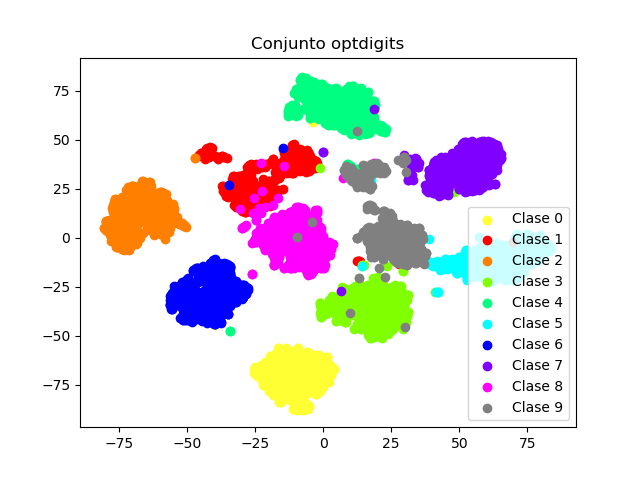
\includegraphics[scale=0.8]{./Imagenes/datos_tsne.png}
	\caption{Datos dibujados como proyección 2D}
\end{figure}

Como podemos observar en el intento de dibujo de los datos éstos están claramente bien separados en clusters y el espacio queda separable de forma muy satisfactoria. Es por esto que el preprocesamiento no se hace necesario en este caso pues los datos de por sí ya son suficientemente buenos como para la aplicación de todas las técnicas que conocemos y hemos estudiado.

Por tanto el modelo final que he decido ajustar es Regresión Logística y por tanto este es en el que vamos a ajustar los parámetros.

Yo he decidido tomar los siguientes:

\begin{itemize}
	\item max\_iter: Número máximo de iteraciones tomado 10.000
	\item tol: tolerancia, tomado $10^-5$
	\item C: parámetro de regularización, tomado 1.0
	\item random\_state: semilla de generación aleatoria, tomada 123456789
	\item solver: algoritmo usado para la minimización interna del error. En este caso lbfgs.
	\item multi\_class: tipo de esquema para clasificación con varias clases, tomado multinomial.
	\item verbose: información por pantalla del algoritmo.
\end{itemize}

Como resultado final he conseguido obtener 0.9521 de score lo cual es un poco menor que en el caso anterior (probablemente por cuestiones de generación aleatoria). 

\subsection{Idoneidad de la métrica usada en el ajuste}

La métrica usada para la evaluación de los resultados es tomar el conjunto de train y entrenar el modelo seleccionado y realizar una predicción de los datos de test para posterior comparación. 

Por tanto la métrica de evaluación es comparar las etiquetas reales con las predichas por el modelo y obtener el tanto por 1 de acierto de la predicción sobre los datos reales.

Esta métrica no es una métrica del todo idónea pues no se tienen en cuenta los fallos de los falsos positivos contra los falsos negativos.

Para entender esta métrica debemos primero definir los conceptos de precisión y exhaustividad.

$$precision = \frac{tp}{tp+fp}$$

$$exhaustividad = \frac{tp}{tp+fn}$$

Donde $tp$ es los verdaderos positivos, $fp$ falsos positivos y $fn$ falsos negativos.

El score F1 es la media armónica de la precisión y la exhaustividad, esto es:

$$F_1 = 2\cdot \frac{precision\cdot exhaustividad}{precision + exhaustividad}$$

Esto se realiza para cada una de las clases, por lo que podemos obtener el score separado o hacer la media. Veamos los resultados:

\begin{table}[H]
	\begin{tabular}{|c|c|c|}
		\hline
		\multirow{2}{*}{{\ul Algoritmo}} & \multicolumn{2}{c|}{{\ul Medidas}} \\ \cline{2-3} 
		& {\ul Acierto}   & {\ul Media F1}   \\ \hline
		\textbf{Logistic Regression}     & 0.9521          & 0.9583           \\ \hline
	\end{tabular}
\end{table}

\begin{table}[H]
	\begin{tabular}{|c|c|c|l|l|l|l|l|l|l|l|}
		\hline
		\multirow{2}{*}{{\ul Algoritmo}} & \multicolumn{10}{c|}{{\ul Medidas}}                                                                                                       \\ \cline{2-11} 
		& {\ul F1 C0} & {\ul F1 C1} & {\ul F1 C2} & {\ul F1 C3} & {\ul F1 C4} & {\ul F1 C5} & {\ul F1 C6} & {\ul F1 C7} & {\ul F1 C8} & {\ul F1 C9} \\ \hline
		\textbf{LR}                      & 0.9909      & 0.9343      & 0.9673      & 0.9516      & 0.9510      & 0.9638      & 0.9810      & 0.9800      & 0.9311      & 0.9583      \\ \hline
	\end{tabular}
\end{table}

Como podemos observar aquí tenemos el score desgranado por clases. Podemos deducir que hemos acertado más en la clase 0 y en la clase 7, por lo que suponemos que la complejidad de detectar estos dígitos es menor para el clasificador. Los dígitos más complejos y por tanto en los que más fallamos son el 1 y el 8, por lo que suponemos que son los que más complejidad presentan. El score F1 medio ha sido de 0.9583 por lo que el score que nos provee sklearn y el propio F1 nos arrojan una información similar. 

\subsection{Estimación de $E_{out}$}

La estimación del error fuera de la muestra la podemos obtener a partir del acierto que hemos obtenido en el apartado anterior. En el caso de regresión logística que ha resultado ser el mejor de nuestros modelos hemos obtenido un tanto por uno de acierto de 0.9521 en el conjunto de test. En nuestro caso el conjunto de train es el tomado como la muestra y por tanto para poder calcular el error fuera de la muestra nos basaremos en el conjunto de test. Si el acierto fuera de la muestra es de 0.9521 entonces el error fuera de la muestra será $1-0.9521 = 0.0479$.

\subsection{Justificación del modelo y calidad del mismo}

Por tanto, por los resultados obtenidos considero que el modelo ofrece una buena calidad pues obtenemos un error fuera de la muestra pequeño, o lo que es lo mismo,  un acierto fuera de la muestra alto.

La calidad del modelo, viene del hecho de que, como ya hemos razonado anteriormente, el conjunto de datos era fácilmente separable por lo que casi todos los algoritmos que hemos estudiado en clase han dado unos resultados parejos siendo quizás el más descolgado el algoritmo Perceptrón.

\section{Problema airfoil: regresión}

\subsection{Problema a resolver}

Tenemos un conjunto de datos llamado ``Airfoil Self-Noise'' que contiene datos de tests aerodinámicos y acústicos. Tiene 5 atributos y una salida continua. Nuestro objetivo a resolver en este problema es intentar ajustar una función que prediga los valores de esta salida continua.

En este conjunto de datos no tenemos tantos datos en la descripción como en el caso de clasificación. Sabemos que todos los atributos son reales, que tiene 1503 instancias con 6 atributos cada una. Este hecho será de relevancia en el estudio pues tenemos muy pocos atributos y deberemos pensar en alguna técnica de aumento de atributos.

\subsection{Preprocesado de los datos}

En este caso no podemos aplicar la reducción de dimensionalidad del ejercicio anterior pues carcería de sentido al disponer ya de muy pocos atributos. Por contra necesitaremos aplicar alguna técnica que nos permita añadir información.

En primer lugar he probado tres procesamientos que son la estandarización, la normalización y la combinación de estos dos de la forma estandarización y después normalización. 

Tal y como he explicado anteriormente la normalización es un preprocesado que nos hace que cada vector que representa una instancia tenga norma 1 y la estandarización nos hace que el conjunto tenga media 0 y lo escalamos mediante la varianza.

Es decir, $z = \frac{x-\bar{x}}{\sigma}$ donde $\bar{x}$ es la media del conjunto y $\sigma$ es la varianza.

Por último y en referencia a añadir nuevos atributos he decidido aplicar una generación polinómica de atributos. Esta generación hace lo siguiente, toma los atributos como variables independientes y añade todos los polinomios de orden el grado que le pasemos como atributo y de orden inferior.

Por ejemplo si tenemos $(X_1 , X_2)$ como vector de características entonces se convierte en $(1,X_1,X_2,X_1^2,X_1\cdot X_2,X_2^2)$

De igual forma si tuviéramos tres características $(X_1,X_2,X_3)$ se convierte en:

$(1,X_1,X_2,X_3,X_1\cdot X_2,X_1\cdot X_3,X_2\cdot X_3,X_1\cdot X_2\cdot X_3, X_1^2, X_1^2\cdot X_2, X_1^2\cdot X_3, X_2^2\cdot X_1, X_2^3\cdot X_3, X_3^2\cdot X_1, X_3^2\cdot X_2, X_1^3, X_2^3, X_3^3)$

Esta construcción no está pensada al tuntún. El hecho de haber incluído no sólo las potencias de los valores, si no además los polinomios mixtos constituye una estructura de anillo de polinomios sobre las variables $(X_1, X_2, X_3)$. Esta construcción además resulta de alto interés porque no sólo añade información extra de cada una de las variables, si no que también añade información interrelacionada de las variables entre sí gracias a los polinomios de variables mixtas.

Tras el estudio de esta aplicación he decidido que el mejor grado es 3 para este conjunto de datos, pues si ponemos menor grado no obtenemos beneficio alguno al aplicar la técnica y si tomamos un grado mayor añadimos complejidad excesiva e información redundante que hace que los regresores obtengan resultados de peor calidad. Además tenemos la capacidad de elegir si tomar sólamente los polinomios mixtos o todos incluídos los que tengan alguna potencia de una variable. En este caso he tomado todos los polinomios porque parece que la información que aportan las potencias es de mayor valor que la que aportan los términos mixtos.

Tras aplicar este proceso he decidido estudiar también el comportamiento de los regresores con este conjunto de datos tras la transformación polinómica y aplicando un esquema de normalización, estandarización y estandarización+normalización.

Como preprocesado extra he decidido aplicar transformaciones de tipo logarítmicas y raíces cuadradas a los datos para estudiar si el comportamiento mejora tras el procesado. 

Con estas tranformaciones he probado a ponerlas solas, junto con estandarizado y junto con generación polinómica de valores.

\subsection{Selección de clases de funciones}

En este caso se nos pide por parte del enunciado del problema que empleemos modelos lineales, esto es modelos que intenten ajustar una función que sea una transformación lineal de los atributos. Por tanto la clase de funciones viene prefijada y por tanto $\mathcal{H}$ viene dada por las fuciones de la forma $h(x) = w_0 + w_1 x_1 + ... + w_d x_d \in \mathcal{H}$.

\subsection{Conjuntos de training, test y validación}

Para los conjuntos de training y test he decidido tomar un esquema de 80\% de train y 20\% de test. Además cabe decir que en este caso como es lógico no podemos utilizar el parámetro stratify para mantener la proporción de las clases pues no tenemos clases, tenemos una salida continua. De esta forma la división no es atendiendo a la salida si no completamente aleatoria manteniendo la proporción 80/20.

\subsection{Regularización, necesidad e implementación}

No necesitamos regularización pues como veremos el modelo no consigue unos datos excesivamente buenos y necesitaremos retocar los parámetros de los modelos para poder escoger uno.

En algunos modelos viene ya implementado por defecto un parámetro de regularización que luego estudiaremos cuando seleccionemos el modelo y deberemos ajustar pues en un principio puede que requiramos una regularización más débil para intentar ajustar un poco mejor los datos.

\subsection{Modelos usados y parámetros empleados}

Para empezar he probado muchos modelos distintos de regresión para intentar ajustar un poco mejor el modelo que mejor se comporta y poder mejorar sus parámetros. Veamos primero cómo se comportan estos modelos sin ningún tipo de preprocesamiento ni ajuste sobre ellos para estudiar un grupo en el que nos debamos de centrar.

En primer lugar cabe decir que los modelos que he considerado inicialmente son:

\begin{itemize}
	\item Mínimos cuadrados
	\item Ridge
	\item Lasso
	\item ElascticNet
	\item Lars
	\item Lasso-Lars
	\item Bayesian Ridge
\end{itemize}

Los resultados base sin preprocesamiento que he obtenido han sido:

\begin{itemize}
	\item Mínimos cuadrados: 0.5258141274677205
	\item Ridge: 0.49993986395648293
	\item Lasso: 0.32299676200104666
	\item ElascticNet: 0.274949699291239
	\item Lars: 0.02588676498032294
	\item Lasso-Lars: 0.5138949582589636
	\item Bayesian Ridge: 0.5047234366540709
\end{itemize}

Posteriormente analizaremos esta métrica en profundidad pero por el momento nos vale con saber que el mejor valor es 1 y a partir de 0 cualquier valor negativo significa que ajusta peor incluso que un hiperplano. 

De esta forma podemos ver que Lars puede ser eliminado del estudio pues es a priori el que muestra un desmarque más significativo entre él y el resto de algoritmos. También vemos que Lasso y ElasticNet obtienen unos resultados pobres pero veremos cómo mejoran con el preprocesamiento.

Por tanto ya estamos en disposición de explicar los modelos que vamos a utilizar. 

\begin{itemize}
	\item Mínimos cuadrados: este modelo intenta ajustar una función lineal, esto es un vector de pesos $w$ de forma que se minimice la suma de los residuos al cuadrado. Esto es en términos generales como decir que la recta y los verdaderos puntos mantengan la mínima distancia o lo que es lo mismo que los errores entre la recta y el verdadero punto se mantengan al mínimo posible.
	\item Ridge: este método sigue la misma base matemática que mínimos cuadrados pues continúa intentando minimizar el factor $min_w || Xw-y ||_2^2$ pero ahora se añade un coeficiente de regularización. Esta regularización es denominada regularización de Tikhonov y que en este caso en la implementación de Scikit Learn se ha tomado como $\alpha ||w||_2^2$ por lo que el modelo completo quedaría como:
	
	$$min_w || Xw-y ||_2^2 + \alpha ||w||_2^2$$ donde $\alpha\geq 0$ es un parámetro que se puede controlar y que si se hace 0 convierte al método Ridge en el propio mínimos cuadrados.
	\item Lasso: este modelo también nace partiendo del modelo de mínimos cuadrados. Lasso intenta minimizar $min_w \frac{1}{2\cdot n_{samples}}||Xw-y||_2^2 + \alpha ||w||_1$. Como podemos ver comparte el término $||Xw-y||_2^2$ como es lógico con mínimos cuadrados. Además este método provee como Ridge un factor de regularización que en el caso de Scikit Learn se ha implementado como $\lambda ||w||_1$ donde $w$ es el vector de pesos que estamos ajustando y $\lambda$ es un parámetro ajustable. Además de este factor de regularización escalamos por el número de muestras. Como diferencia también con Ridge estamos tomando en el factor de regularización la norma $L1$ en vez de la $L2$, es decir, $||w||_1 = \sum_{i=1}^{n}|w_i|$. 
	\item ElascticNet: ElasticNet toma la base de mínimos cuadrados, Lasso y Ridge intentando hacer una combinación adecuada de estos métodos de regularización. La forma que queremos minimizar ahora es $min_w \frac{1}{2n_{samples}}|| Xw-y ||_2^2 + \alpha \rho ||w||_1 + \frac{\alpha (1-\rho)}{2}||w||_2^2$. La ventaja que estamos viendo es la combinación de la ponderación de la norma $L1$ y $L2$ que incorporaban de forma independiente Lasso y Ridge. La complejidad del modelo asciende pues ahora tenemos los parámetros de Ridge y los de Lasso pero comprobaremos que el comportamiento está a la altura del resto de algoritmos. Esta combinación nació como solución a algunas flaquezas que los modelos Ridge y Lasso presentaban de forma separada pero no las sufren con una combinación adecuada.
	\item Lasso-Lars: LARS es un paradigma nuevo de regresión que intenta en vez de minimizar únicamente los errores, mantener una relación de ángulos entre la recta propuesta y los puntosdel espacio. El modelo LARS es el que hemos descartado anteriormente pues funcionaba mal. La idea es que LARS está pensado para alta dimensionalidad mientras que Lasso no, por lo tanto la combinación del método LARS con la regularización propuesta por Lasso hace que se mejore el comportamiento haciendo interesante considerar este método.
	\item Bayesian Ridge: este modelo intenta utilizar conocimiento del área de la inferencia bayesiana junto con el modelo de regresión Ridge. Las probabilidades ahora de $w$ vienen dadas por una distribución esférica gaussiana. Los parámetros $\alpha$ y $\lambda$ vienen dados por una distribución gamma. De esta forma se intenta hacer una estimación de los parámetros mediante estas distribuciones para ajustar mejor los modelos a los datos.
\end{itemize}

Veamos los resultados de los modelos:

\begin{table}[H]
	\begin{tabular}{|c|c|c|c|c|c|c|}
		\hline
		\multirow{2}{*}{{\ul Preprocesamiento}}                              & \multicolumn{6}{c|}{{\ul Algoritmos}}                                                             \\ \cline{2-7} 
		& {\ul MC} & {\ul Ridge} & {\ul Lasso} & {\ul ElasticNet} & {\ul Lasso-LARS} & {\ul Bayesian Ridge} \\ \hline
		\textbf{Sin}                                                         & 0.5034   & 0.4877      & 0.3170      & 0.2495           & 0.4917           & 0.2474               \\ \hline
		\textbf{\begin{tabular}[c]{@{}c@{}}Raiz cuadrada\\ (R)\end{tabular}} & 0.4935   & 0.4898      & 0.4046      & 0.2521           & 0.4975           & 0.4926               \\ \hline
		\textbf{Logaritmo(L)}                                                & 0.4416   & 0.3842      & 0.2145      & 0.1151           & 0.4438           & 0.4422               \\ \hline
		\textbf{L+E}                                                         & 0.4706   & 0.4706      & 0.4588      & 0.2966           & 0.4610           & 0.4688               \\ \hline
		\textbf{R+E}                                                         & 0.5023   & 0.5024      & 0.5034      & 0.3613           & 0.5042           & 0.5033               \\ \hline
		\textbf{P+R+E}                                                       & 0.7940   & 0.7735      & 0.6486      & 0.5937           & 0.6504           & 0.7037               \\ \hline
		\textbf{P+L+E}                                                       & 0.4925   & 0.7300      & 0.5806      & 0.4727           & 0.5846           & 0.7204               \\ \hline
		\textbf{Estandarizado (E)}                                           & 0.5013   & 0.5013      & 0.4889      & 0.3045           & 0.4909           & 0.5009               \\ \hline
		\textbf{Normalización (N)}                                           & 0.1526   & 0.0678      & -0.004      & -0.004           & 0.1341           & 0.1319               \\ \hline
		\textbf{Polinómica}                                                  & 0.5483   & 0.6627      & 0.6612      & 0.6541           & 0.6180           & 0.5134               \\ \hline
		\textbf{P+E}                                                         & 0.6861   & 0.7003      & 0.6255      & 0.5717           & 0.6263           & 0.6371               \\ \hline
		\textbf{P+N}                                                         & -2.8666  & 0.0765      & -0.0004     & -0.0004          & 0.1560           & 0.17833              \\ \hline
		\textbf{P+N+E}                                                       & 0.1246   & 0.1255      & 0.1158      & 0.0153           & 0.1231           & 0.1312               \\ \hline
		\textbf{N+E}                                                         & -20.6287 & -0.1940     & 0.1400      & 0.0694           & 0.1387           & -0.6916              \\ \hline
	\end{tabular}
\end{table}

El mejor escenario y puntuación para cada algoritmo ha sido:

\begin{table}[H]
	\begin{tabular}{|l|l|l|}
		\hline
		\multirow{2}{*}{{\ul Algoritmos}} & \multicolumn{2}{l|}{{\ul Mejor combinación}}              \\ \cline{2-3} 
		& {\ul Procesamiento}                         & {\ul Score} \\ \hline
		\textbf{Mínimos cuadrados}        & Polinómica + Raíz cuadrada+ estandarización & 0.7940      \\ \hline
		\textbf{Ridge}                    & Polinómica + Raíz cuadrada+ estandarización & 0.7735      \\ \hline
		\textbf{Lasso}                    & Polinómica                                  & 0.6612      \\ \hline
		\textbf{ElasticNet}               & Polinómica                                  & 0.6541      \\ \hline
		\textbf{Lasso-LARS}               & Polinómica + Raíz cuadrada+ estandarización & 0.6504      \\ \hline
		\textbf{Bayesian Ridge}           & Polinómica + Raíz cuadrada+ estandarización & 0.7204      \\ \hline
	\end{tabular}
\end{table}

Como podemos observar el algoritmo que mejor score nos ha dado ha sido mínimos cuadrados que nos arroja un 79.40\% de acierto en la métrica $R^2$ que nos proporciona Sklearn por defecto. 

Estudiemos y ajustemos un poco más el modelo.

\subsection{Selección y ajuste del modelo final}

\subsection{Idoneidad de la métrica usada en el ajuste}

\subsection{Estimación de $E_{out}$}

\subsection{Justificación del modelo y calidad del mismo}

\end{document}
